\clearpage
\subsection{Cross-store curves}\label{sec:curves}
These five figures retain the historical full-matrix/external populations, not run-9 measurements. The new matched-caller grid is in Section~\ref{sec:rwc}.

\begin{figure}[H]\centering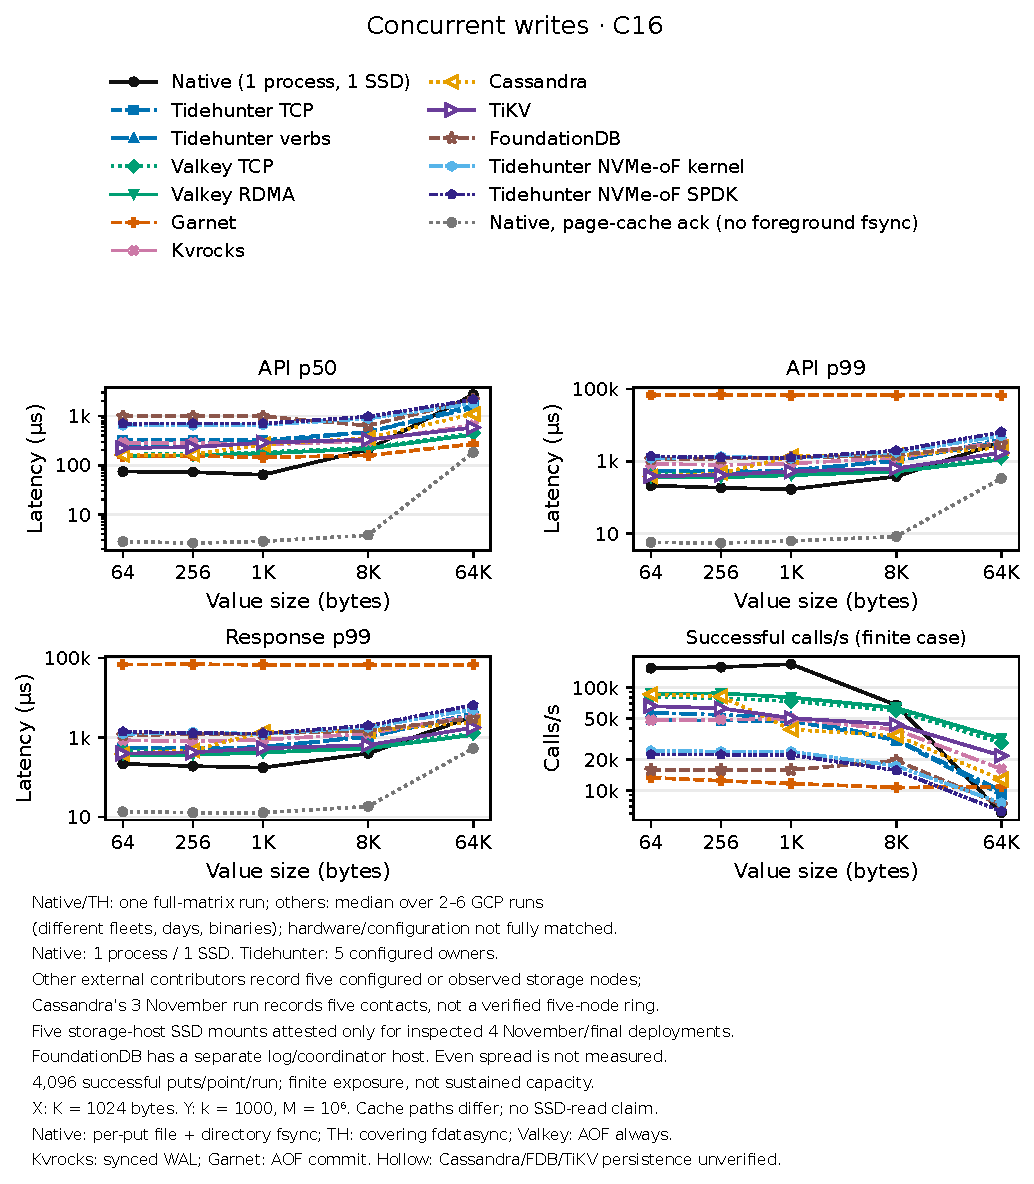
\includegraphics[width=\linewidth]{figures/curves-write-c16.pdf}
\caption{Verified series: Class B, synced before acknowledgement. \ackUnknown\ Separate grey Native Class A: \texttt{native\_async\_write}, page cache, no foreground fsync; finite rate omitted. Scalar puts, c16. Primary RF1; \N{curve:write-concurrent:put:calls} successful puts/run. \runs. Sync mechanics and topology differ; no cross-class ranking.}\label{fig:curves-write}
\end{figure}
At 1 KiB, synchronous verbs p50 is \N{p50:th_verbs:primary_rf1:write-concurrent:put:1024|.1f}~\us; historical Valkey RDMA AOF-always p50 is \N{p50:valkey_rdma:primary_rf1:write-concurrent:put:1024|.1f}~\us. At 64 KiB, Native's one-SSD per-put barrier has p50 \N{p50:native:primary_rf1:write-concurrent:put:65536|.1f}~\us; five-owner synchronous verbs has \N{p50:th_verbs:primary_rf1:write-concurrent:put:65536|.1f}~\us. Section~\ref{sec:native-gap} explains the topology and acknowledgement mismatch; the plot does not isolate their costs.

\clearpage
\begin{figure}[H]\centering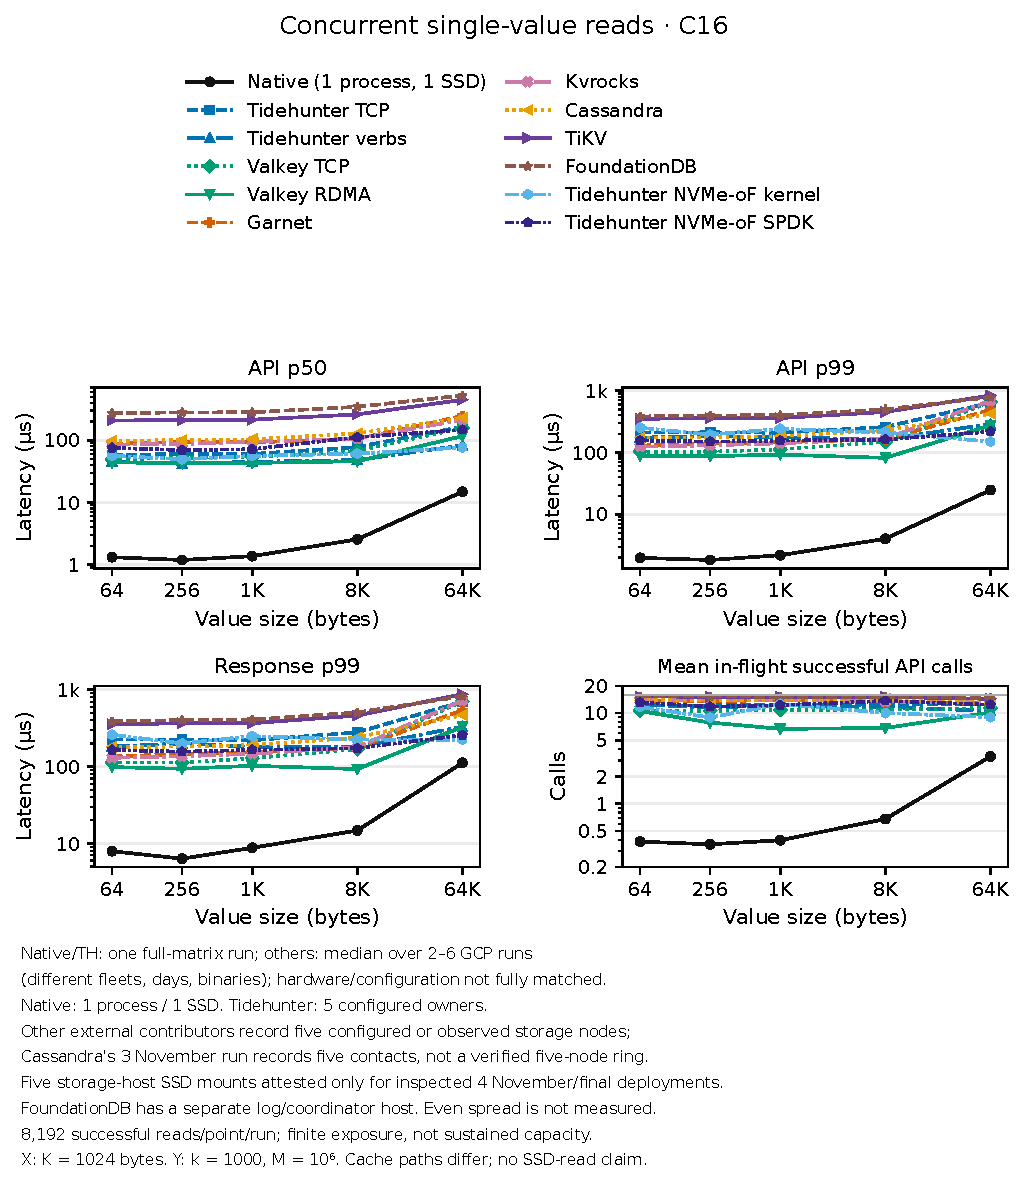
\includegraphics[width=\linewidth]{figures/curves-read-c16.pdf}
\caption{\ackB\ \ackUnknown\ Single-value reads, primary RF1, c16. Each point: \N{curve:read-concurrent:read:calls} successful reads/run. \runs. Panel four shows mean in-flight successful API calls per run, then the external median. The grey line marks 16 workers; it is not a store series. Cache paths differ; no SSD-latency ranking follows.}\label{fig:curves-read}
\end{figure}
At 64 KiB, owner verbs resident-oriented read p50 is \N{p50:th_verbs:primary_rf1:read-concurrent:read:65536|.1f}~\us, versus historical Valkey RDMA RAM GET \N{p50:valkey_rdma:primary_rf1:read-concurrent:read:65536|.1f}~\us. Native's resident-oriented p50 is \N{p50:native:primary_rf1:read-concurrent:read:65536|.1f}~\us; its low occupancy means its case rate is not a capacity estimate. Owner TCP includes mutual TLS; trusted verbs does not.

\clearpage
\begin{figure}[H]\centering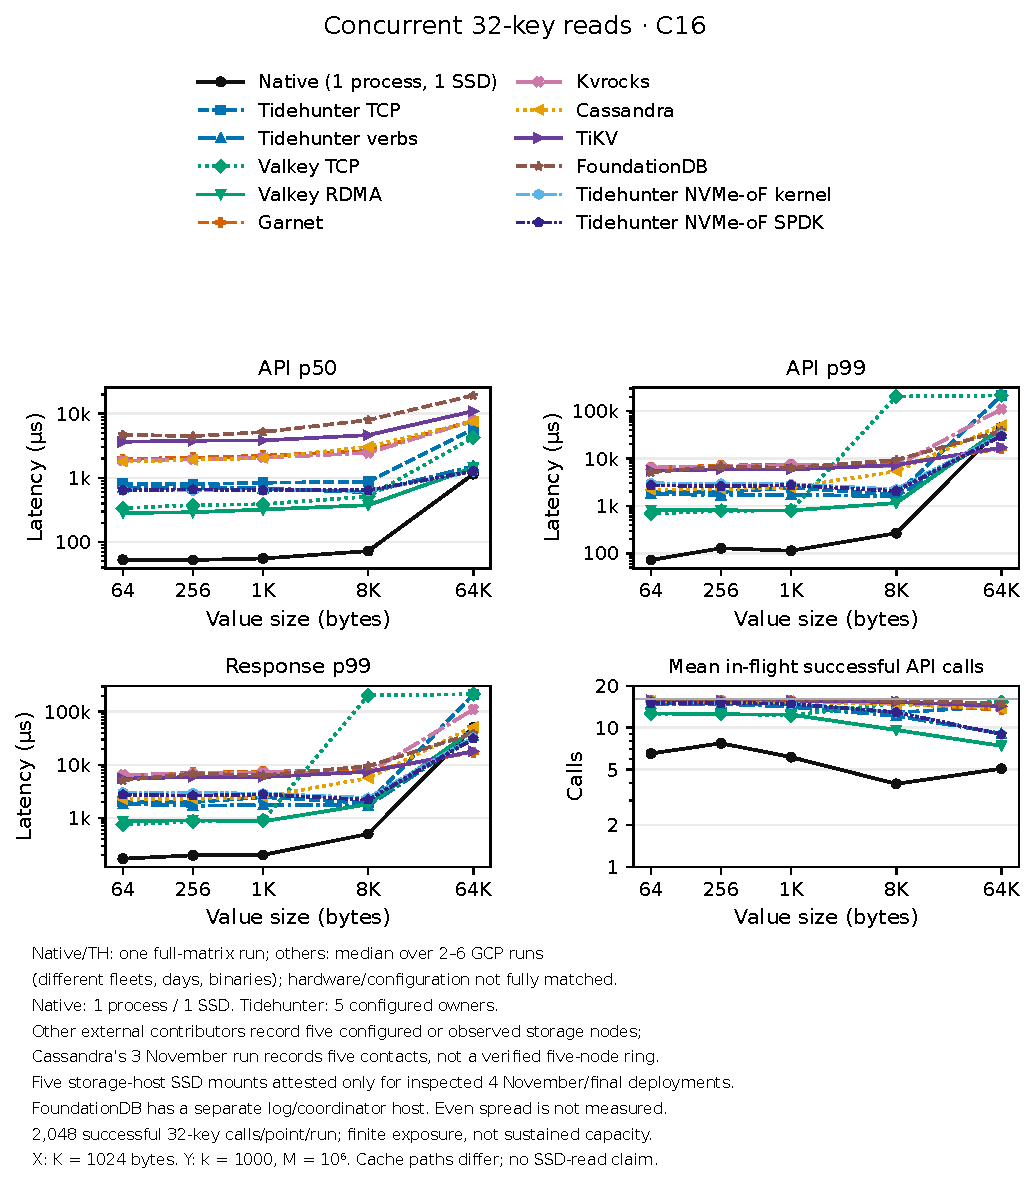
\includegraphics[width=\linewidth]{figures/curves-read32-c16.pdf}
\caption{\ackB\ \ackUnknown\ 32-key reads, primary RF1, c16. Each point: \N{curve:read-many32:get_many:calls} successful calls/run, each for 32 keys. \runs. Panel four shows mean in-flight successful API calls per run, then the external median. The grey line marks 16 workers; it is not a store series. It counts calls, not keys. Read caches differ.}\label{fig:curves-read32}
\end{figure}
At 1 KiB per value, owner verbs resident-oriented p50 is \N{p50:th_verbs:primary_rf1:read-many32:get_many:1024|.1f}~\us; historical Valkey RDMA RAM-read p50 is \N{p50:valkey_rdma:primary_rf1:read-many32:get_many:1024|.1f}~\us. At 64 KiB per value, verbs p99 is \N{p99ms:th_verbs:primary_rf1:read-many32:get_many:65536|.1f}~ms versus Valkey RDMA \N{p99ms:valkey_rdma:primary_rf1:read-many32:get_many:65536|.1f}~ms. Native uses one local SSD and a resident-oriented workload; these are not matched cold-device calls.

\clearpage
\begin{figure}[H]\centering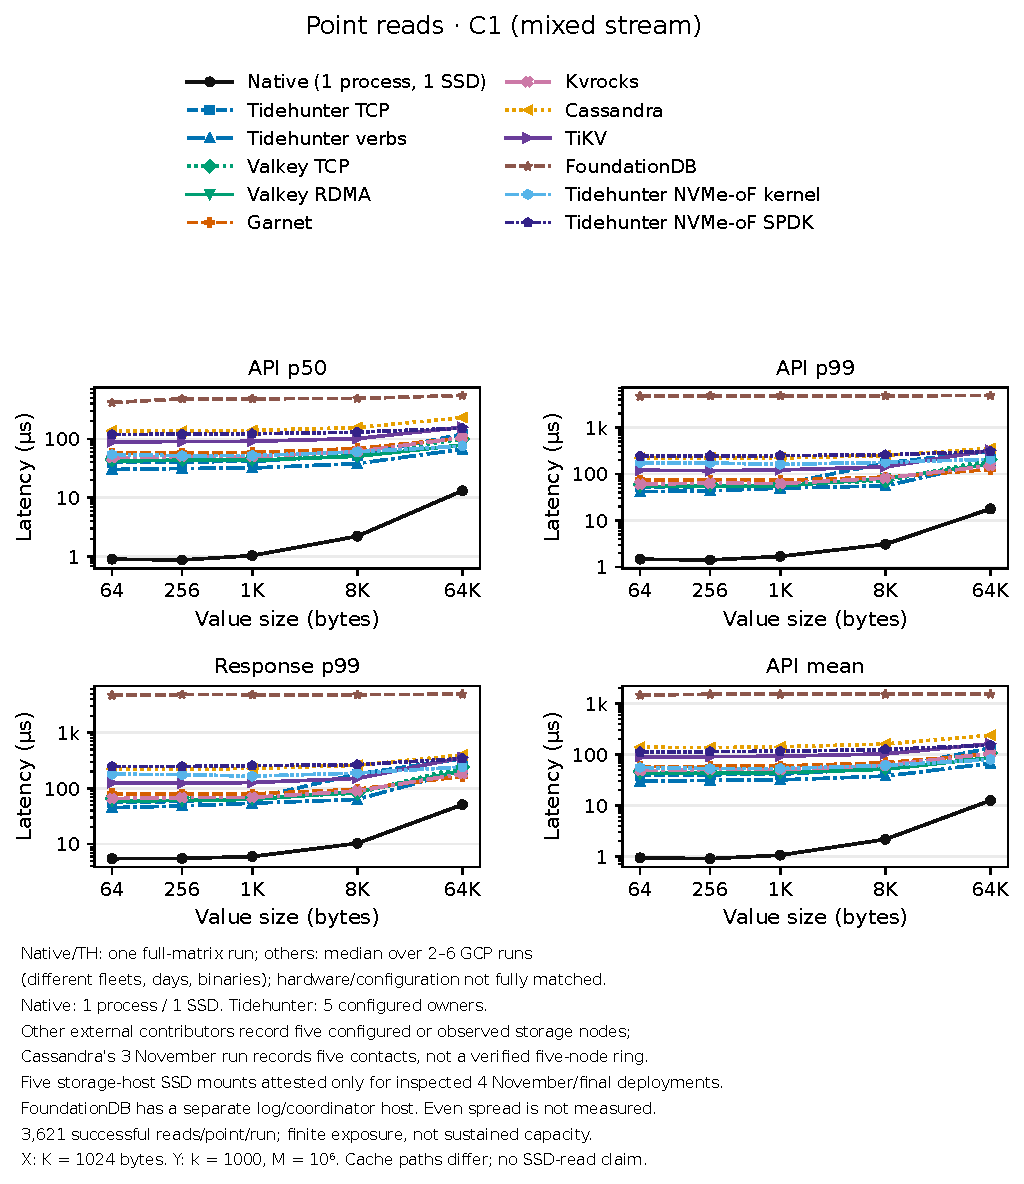
\includegraphics[width=\linewidth]{figures/curves-point-read-c1.pdf}
\caption{\ackB\ \ackUnknown\ Point reads at c1 within a mixed stream. Each latency point: \N{curve:point-mixed:read:calls} successful reads/run in a \N{curve:point-mixed:read:case_calls}-call case with puts, deletes and missing reads. \runs. Panel four shows read API mean, not mixed-case throughput. Cache paths differ.}\label{fig:curves-point-read}
\end{figure}
At 1 KiB, owner verbs resident-oriented p50 is \N{p50:th_verbs:primary_rf1:point-mixed:read:1024|.1f}~\us, versus historical Valkey RDMA RAM GET \N{p50:valkey_rdma:primary_rf1:point-mixed:read:1024|.1f}~\us. At 64 KiB, the corresponding p50 values are \N{p50:th_verbs:primary_rf1:point-mixed:read:65536|.1f} and \N{p50:valkey_rdma:primary_rf1:point-mixed:read:65536|.1f}~\us. This mixed stream is not the read-only c16 workload; it does not isolate concurrency scaling.

\clearpage
\begin{figure}[H]\centering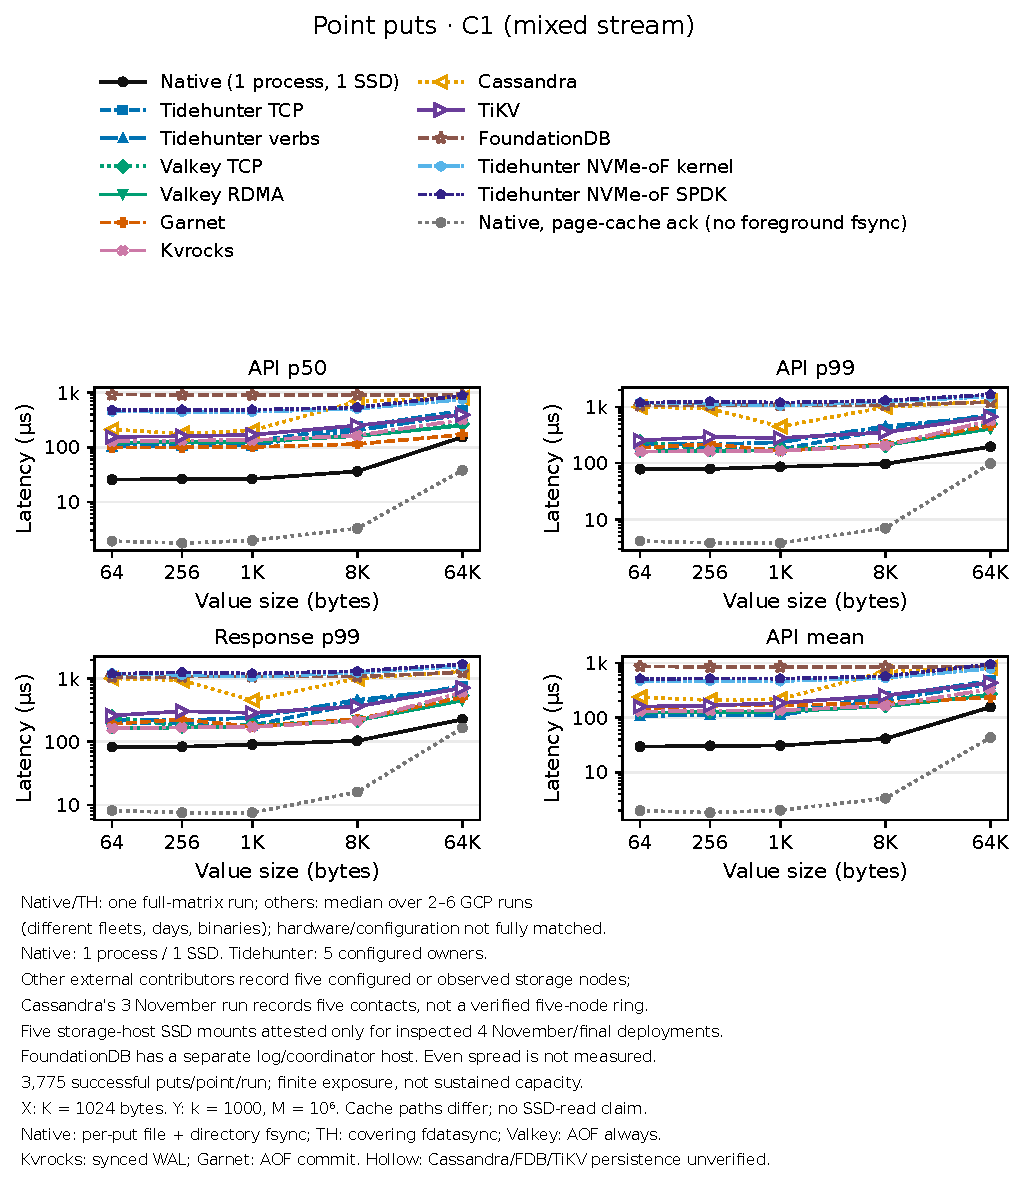
\includegraphics[width=\linewidth]{figures/curves-point-put-c1.pdf}
\caption{\ackB\ \ackUnknown\ Point puts at c1 within a mixed stream. Each latency point: \N{curve:point-mixed:put:calls} successful puts/run in a \N{curve:point-mixed:put:case_calls}-call case. \runs. Panel four shows put API mean. Grey dotted Native is a separate Class A page-cache reference; it has no per-put foreground fsync or per-put persistence guarantee; hollow markers mean unverified device persistence.}\label{fig:curves-point-put}
\end{figure}
At 1 KiB, owner synchronous verbs p50 is \N{p50:th_verbs:primary_rf1:point-mixed:put:1024|.1f}~\us; historical Valkey RDMA AOF-always p50 is \N{p50:valkey_rdma:primary_rf1:point-mixed:put:1024|.1f}~\us. At 64 KiB, those values are \N{p50:th_verbs:primary_rf1:point-mixed:put:65536|.1f} and \N{p50:valkey_rdma:primary_rf1:point-mixed:put:65536|.1f}~\us; Native's one-SSD per-put barrier is \N{p50:native:primary_rf1:point-mixed:put:65536|.1f}~\us. Different fsync mechanics, topology and fleets prevent a transport-only or matched-durability ranking.
